%中間審査概要テンプレート ver. 3.0

\documentclass[uplatex,twocolumn,dvipdfmx]{jsarticle}
\usepackage[top=22mm,bottom=22mm,left=22mm,right=22mm]{geometry}
\setlength{\columnsep}{10mm}
\usepackage[T1]{fontenc}
\usepackage{txfonts}
\usepackage[expert,deluxe]{otf}
\usepackage[dvipdfmx,hiresbb]{graphicx}
\usepackage[dvipdfmx]{hyperref}
\usepackage{pxjahyper}
\usepackage{secdot}





%タイトルと学生番号,名前だけ編集すること
\title{\vspace{-5mm}\fontsize{14pt}{0pt}\selectfont 文書自動添削システムによる学生の文書改善履歴の調査}
\author{\normalsize プロジェクトマネジメントコース 矢吹研究室 1442031 氏名 小山隆太郎}
\date{}
\pagestyle{empty}
\begin{document}
\fontsize{10.5pt}{\baselineskip}\selectfont
\maketitle





%以下が本文
\section{背景}
学生が行う研究では,研究だけではなく文書を作成する時間が多い.特に卒業論文は文量も多く,形式も指定されるため,文書校正にかかる労力は大きい.また,自分以外が読んでもわかりやすい文書を書く必要があり,文が長いほど理解が難しくなってしまう場合や,「だから」,「かなり」といった口語が混じり,文書の質が落ちてしまうことがある.

このような状況にRedPen\cite{a}を執筆環境に導入することで,文書の質が向上することが期待されている.RedPenは技術文書をターゲットにした文書自動添削ツールであり,現在もコードの追加,改変が行われている.

\section{目的}
RedPenは学校や会社等の組織のルールに対応できるように設定が柔軟に行える仕様になっている.マシンを用いた文書添削を繰り返し行い,論文向けの添削システムを確立し,文書の質の向上と,作成時間の短縮を図ることを目的とする.

\section{手法}
添削システムに必要な要素を以下の手法で調査する.

\begin{enumerate}
 \item 執筆中の文書の添削に,CI(継続的インテグレーション)サーバを導入する\cite{b}.
 \item GitHubに文書をアップロードするとWerckerが自動で動作するようにし,添削結果を出力する.
 \item 添削結果を記録し,添削システムに必要な要素を考察し,RedPenのコードを追加,改変する.
\end{enumerate}

\section{想定される成果物}
個人,複数人プロジェクトで活用できる文書添削システムを構築する.

\section{進捗状況}
矢吹研究室に所属する3年生の課題文を添削を行った際の,エラー数の推移は図\ref{conf}のとおりである.各折れ線が文章1本のエラー数の推移を表している.エラー数が減った文書の修正は以下のように行われた.

\begin{enumerate}
 \item 文頭からマルの文字数を120字以内に収め,カンマや同一単語の複数回利用を修正し,文長を短くした.ですます調,数値や専門用語の記述を統一した文書は右下がりの推移を得た
 \item 3回目の添削でエラー数が30個ある文書は,「が」,「と」等の接続詞が連続し,読みにくくなった文書.同一の専門用語が複数回利用され,文長が長くなった文書である
\end{enumerate}

\begin{figure}[h]
\centering
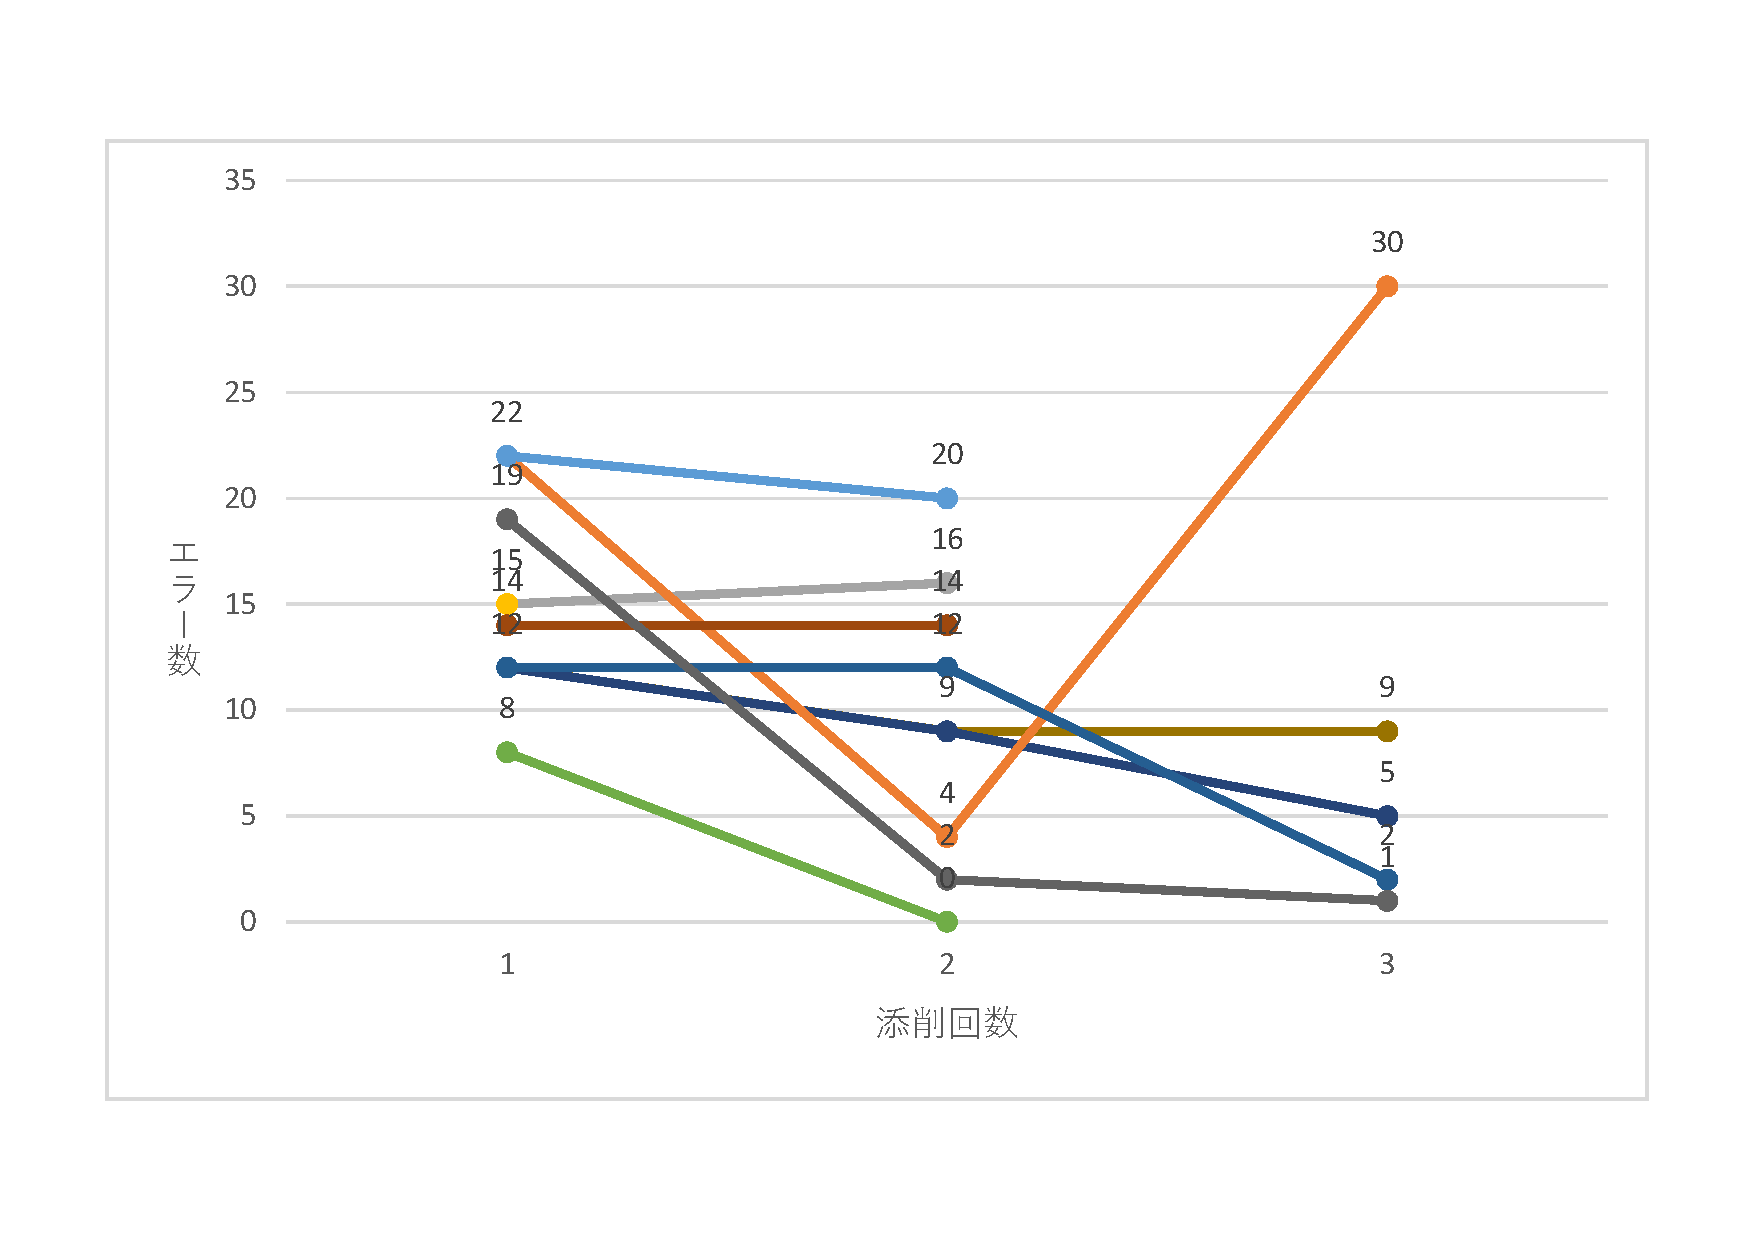
\includegraphics[width=6.5cm,clip]{redpen.pdf}
\caption{添削項数の推移}\label{conf}
\end{figure}

\section{今後の計画}
添削機能が不十分なため,エラー数が減らなかった文書があった.卒論や課題文等を書く学生がより質の良い文書が書けるよう添削マシンを構築する.

\bibliographystyle{junsrt}
\bibliography{biblio}%「biblio.bib」というファイルが必要.


\end{document}
